\documentclass[]{article}
\usepackage{setspace}
\usepackage{amsmath}
\usepackage{geometry}
\usepackage { enumerate }
\usepackage{amssymb}
\usepackage{graphicx}
\graphicspath{ {./images/} }

\geometry{a4paper,scale=0.80}


%opening
\title{Assignment 2}
\author{z5395765}

\begin{document}
	\maketitle

	\begin{spacing}{1.5}

		\section*{Problem1}
		Let S be a set.\\
		(a) Show that for any set T and any function $ f : S \rightarrow T$, the relation $ R_f \subseteq S \times S$, defined as:\\
		\begin{center}
				$ (s, s') \in R_f$ if and only if $f(s) = f(s')$
		\end{center} 
		is an equivalence relation.
		
		\subsection*{Proof of (a)}
		In order to show $ R_f $ is an equivalence relation, I will show that $ R_f $ is reflexive, symmetric and transitive.
		\subsubsection*{(1) Proof of reflexive}
		For all $ s \in S $, we have $ f(s) = f(s) $. Therefore, $ (s, s) \in R_f$, so $ R_f $ is reflexive.
		 \subsubsection*{(2) Proof of symmetric} 
		 Suppose $ (s, s') \in R_f $, then $ f(s) = f(s') $. Therefore, $ f(s') = f(s) $. Therefore, $ (s', s) \in R_f $. So, $ R_f $ is symmetric.
		  \subsubsection*{(3) Proof of transitive}
		  Suppose $ (s, s') \in R_f, (s', s'') \in R_f $, then $ f(s) = f(s')$, $ f(s') = f(s'') $. Therefore, $ f(s) = f(s'') $. Therefore, $ (s, s'') \in R_f $. Therefore, $ R_f $ is transitive.\\
		  In conclusion, the relation $ R_f $ is an equivalence relation.\\
		  ~\\
		(b) Show that if $ R \subseteq S \times S $ is an equivalence relation, then there exists a set T and a function $ f_R : S \rightarrow T $ such that:
		\begin{center}
			$ (s, s') \in R $ if and only if $ f_R(s) = f_R(s') $.
		\end{center}
		\subsection*{Proof of (b)}
		Assume T is set of equivalence classes of R. Suppose $ f_R(x) = [x] $.\\
		Firstly, if $ (s, s') \in R $, according to fact in lecture, then [s] = [s'], so $ f_R(s) = f_R(s') $.\\
		Secondly, if $ f_R(s) = f_R(s') $, then  [s] = [s'], according to fact in lecture, $ (s, s') \in R $.\\
		In conclusion, there exists a set T and a function $ f_R : S \rightarrow T $ such that: $ (s, s') \in R $ if and only if $ f_R(s) = f_R(s') $.
		
		
		\section*{Problem2}
		\subsection*{(a) Show that for all $ a,b \in N: $}
		\subsubsection*{(i) Prove $ f(a+b) = max\{f(a),f(b)\} $}
		If $ a>0,b>0,f(a)=f(b)=1,f(a+b)=1 $, satisfy.\\
		If $ a>0,b=0,f(a)=1,f(b)=0,f(a+b)=1$, satisfy.\\
		If $ a=0,b>0,f(a)=0,f(b)=1,f(a+b)=1 $, satisfy.\\
		If $ a=0,b=0,f(a)=f(b)=0,f(a+b)=0 $, satisfy.\\
		Therefore, for all $ a,b \in N$, $ f(a+b) = max\{f(a),f(b)\} $.
		\subsubsection*{(ii) Prove $ f(ab) = min\{f(a),f(b)\} $}
		If $ a>0,b>0,f(a)=f(b)=1,f(ab)=1 $, satisfy.\\
		If $ a>0,b=0,f(a)=1,f(b)=0,f(ab)=0$, satisfy.\\
		If $ a=0,b>0,f(a)=0,f(b)=1,f(ab)=0 $, satisfy.\\
		If $ a=0,b=0,f(a)=f(b)=0,f(ab)=0 $, satisfy.\\
		Therefore, for all $ a,b \in N$, $ f(ab) = min\{f(a),f(b)\} $.
		\subsection*{(b)}
		\subsection*{(i) Show that $ \boxplus $ is a function.}
		In order to prove $ \boxplus $ is a function, I will show that $ \boxplus $ is Functional and Total.
		\subsubsection*{Proof of Total}
		If $ (X,Y) \in E \times E$, then there is $ x \in N $ such that $ X=[x] $, $ y \in N $ such that $ Y=[y] $. Let $ Z = [x+y] \in E$, then by definition of $ \boxplus $, $ ((x,y),z) \in \boxplus $. Therefore for every $ (X,Y) \in E \times E$, there is at most one $ Z \in E $, such that $ ((X,Y),Z) \in \boxplus $. Therefore, $ \boxplus $ is Total.
		\subsubsection*{Proof of Functional}
		Suppose $ (X,Y) \in E \times E$, $ ((x,y),z) \in \boxplus $, $ ((x',y'),z') \in \boxplus $, then there is x, y such that  $ X=[x], Y=[y], Z = [x+y]$; there is x', y' such that  $ X=[x'], Y=[y'], Z = [x'+y']$. I will show that  if $ [x]=[x'], [y]=[y'] $, then $ [x+y]=[x'+y'], Z=Z' $.\\
		Suppose $ [x]=[x'], [y]=[y'] $, therefore $ x R_f x', y R_f y' $. Therefore, $ f(x)=f(x'), f(y)=f(y') $. Therefore, $ max(f(x),f(y)) = max(f(x'),f(y')) $. Therefore, $ f(x+y) = f(x'+y') $, so $ (x+y) R_f (x'+y') $. Therefore, $ [x+y] = [x'+y']. $Therefore for every $ (X,Y) \in E \times E$, there is at most one $ Z \in E $, such that $ ((X,Y),Z) \in \boxplus $. Therefore, $ \boxplus $ is Functional.\\
		~\\
		In conclusion, $ \boxplus $ is a function.
		\subsection*{(ii) Show that $ \boxdot $ is a function.}
		In order to prove $ \boxdot $ is a function, I will show that $ \boxdot $ is Functional and Total.
		\subsubsection*{Proof of Total}
		If $ (X, Y) \in E \times E$, then there is $ x \in N $ such that $ X=[x] $, $ y \in N $ such that $ Y=[y] $. Let $ Z = [xy] \in E$, then by definition of $ \boxdot $, $ ((x,y),z) \in \boxdot $. Therefore for every $ (X,Y) \in E \times E$, there is at least one $ Z \in E $, such that $ ((X,Y),Z) \in \boxdot $.  Therefore, $ \boxdot $ is Total.
		\subsubsection*{Proof of Functional}
		Suppose $ (X,Y) \in E \times E$, $ ((x,y),z) \in \boxdot $, $ ((x',y'),z') \in \boxdot $, then there is x, y such that  $ X=[x], Y=[y], Z = [xy]$; there is x', y' such that  $ X=[x'], Y=[y'], Z = [x'y']$. I will show that  if $ [x]=[x'], [y]=[y'] $, then $ [xy]=[x'y'], Z=Z' $.\\
		Suppose $ [x]=[x'], [y]=[y'] $, therefore $ x R_f x', y R_f y' $. Therefore, $ f(x)=f(x'), f(y)=f(y') $. Therefore, $ min(f(x),f(y)) = min(f(x'),f(y')) $. Therefore, $ f(xy) = f(x'y') $, so $ (xy) R_f (x'y') $. Therefore, $ [xy] = [x'y'].$ Therefore for every $ (X,Y) \in E \times E$, there is at most one $ Z \in E $, such that $ ((X,Y),Z) \in \boxdot $. Therefore, $ \boxdot $ is Functional.\\
		~\\
		In conclusion, $ \boxdot $ is a function.
		\subsection*{(c) Show that for all $ A,B,C \in E: $}
		\subsubsection*{(i) Prove $ A \boxdot [1] = A$}
		Suppose $ A = [a] $, $ a $ is an arbitrary element in $ N $.\\
		$ A \boxdot [1] = [a] \boxdot [1] = [a \times 1] = [a] = A$.
		\subsubsection*{(ii) Prove $ A \boxplus B = B \boxplus A$}
		Suppose $ A = [a] $, $ B = [b] $, $ a, b $ are arbitrary elements in $ N $.\\
		$ A \boxplus B =  [a] \boxplus [b] = [a+b] = [b+a] = [b] \boxplus [a] = B \boxplus A$.
		\subsubsection*{(iii) Prove $ A \boxdot (B \boxplus C) = (A \boxdot B) \boxplus (A \boxdot C)$}
		Suppose $ A = [a] $, $ B = [b] $, $ C = [c] $, $ a, b, c $ are arbitrary elements in $ N $.\\
		$ A \boxdot (B \boxplus C) = [a] \boxdot ([b] \boxplus [c])  = [a] \boxdot [b+c] = [a(b+c)] = [ab+ac] = [ab]  \boxplus [ac] = ([a] \boxdot [b]) \boxplus ([a] \boxdot [c]) = (A \boxdot B) \boxplus (A \boxdot C)$.
		
		\section*{Problem3}
		\subsection*{(a) Model this as a graph problem. }
		(i) We can model this problem with the following graph:\\
		-Vertices: A vertex for every house\\
		- Edges: An edge between two vertices if the wireless networks of the corresponding houses can interfere, and must therefore be on different channels.\\
		For this particular problem, this would result in the following graph:\\
		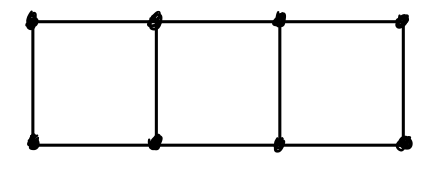
\includegraphics{1}
		~\\
		(ii) If we model each house with a color, then assigning different Internet channels to houses is modelled by coloring vertices. The requirement that the wireless networks of neighbouring houses will interfere then corresponding to no edge having both its endpoints being the same colour. So the problem of finding the minimum number of different channels the neighbourhood requires corresponds to the graph problem of finding the chromatic number of the resulting graph.
		\subsection*{(b) Give the solution to the graph problem corresponding to this scenario; and determine the minimum number of the wi-fi channels required for the neighbourhood.}
		The graph that models our problem is as below. As we can see, the chromatic number of this graph is 2. For example, here is a 2-colouring of the graph:\\
		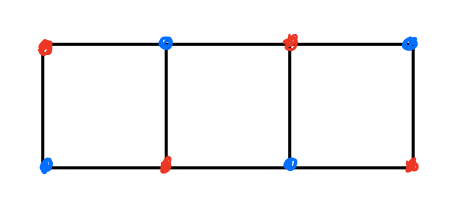
\includegraphics{2}\\
		Therefore, in this scenario, the minimum number of the wi-fi channels required for the neighbourhood is 2.
		\subsection*{(c) How do your answers to (a) and (b) change if a house's wireless network can also interfere with those of the houses to the left and right of the house over the road?}
		If a house's wireless network can also interfere with those of the houses to the left and right of the house over the road, then the resulting graph would look like:\\
		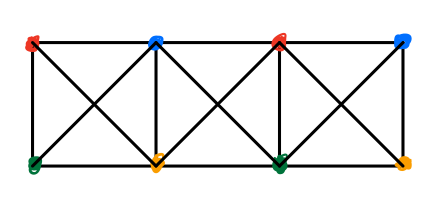
\includegraphics{3}\\
		In this scenario, the minimum number of the wi-fi channels required for the neighbourhood is 4.
		
		
		\section*{Problem4}
		\subsection*{(a) Give an argument to show that the Petersen graph does not contain a subdivision of $ K_5 $}
		Suppose the Petersen graph contains a subdivision of $ K_5 $. Consider transforming the Petersen graph to $ K_5 $ via Strategy II from the lectures. At each step of the transformation we do one of:\\
		- Delete an edge\\
		- Delete a vertex(and all adjacent edges)\\
		- Replace a vertex of degree 2 with an edge connecting its neighbours(contracting a vertex)\\
		For each steps we observe the degree of every vertex decreases or stay the same. However, The degree of every vertices in the Petersen graph is 3 and the degree of every vertices in $ K_5 $  is 4. So it is not possible to tranform the Petersen graph to $ K_5 $ using Strategy II.\\
		Therefore, the Petersen graph does not contain a subdivision of $ K_5 $ .
		
		\subsection*{(b) Show that the Petersen graph contains a subdivision of $ K_{3,3}$}
		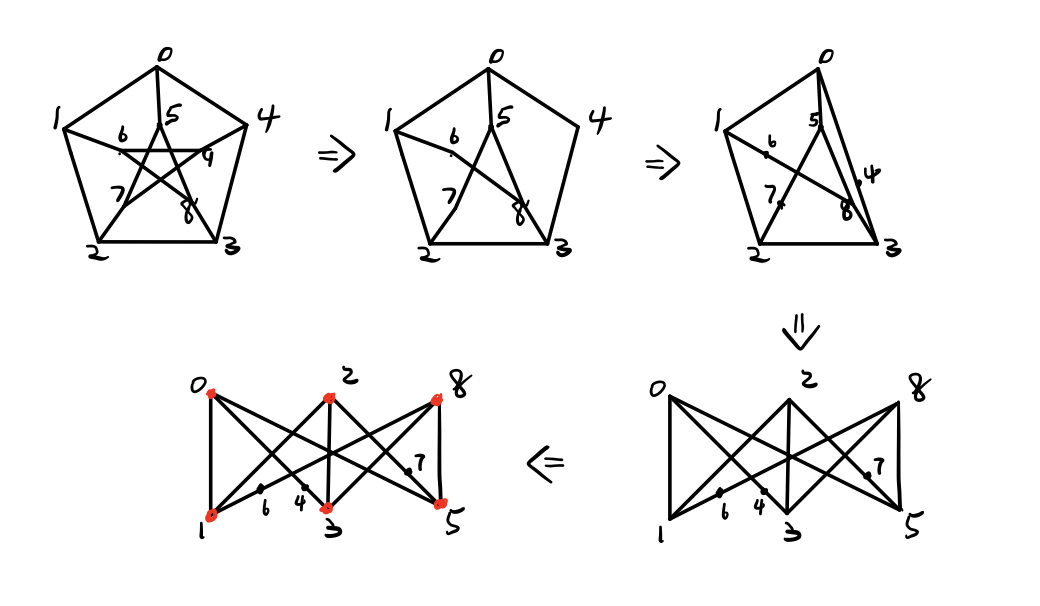
\includegraphics{4}
		
		\section*{Problem5}
		\subsection*{(a) Prove that for all $ i, j \in N $, if $ i \leq j $ then $ R^i \subseteq R^j $}
		Let $ P_i(j) $ be the proposition that $ R^i \subseteq R^j $ and I will prove that $ P_i(j) $ holds for all $ j \geq i $ by induction on $ j $.\\
		Base case: $ i = j $. \\
		Here we have $ R^i = R^j $. So $ P_i(j) $ is true.\\
		Inductive case: \\
		Assume that $ P_i(j) $ holds for some $ i \leq j$ and $i, j \in N $. That is, $ R^i \subseteq R^j $. Then $ R^{j+1}  = R^j \cup (R; R^j)$, so $ R^i \subseteq R^{j+1} $. Therefore, $ P_i(j+1) $ holds.\\
		In conclusion, we have our base case of $ P_i(j) $ holds then $ P_i(j+1) $ holds. Therefore, by induction, $ P_i(j) $ holds for all $ j \geq i $.
		
		\subsection*{(b) Let $ P(n) $ be the proposition that for all $ m \in N: R^n; R^m = R^{n+m} $}		
		I will prove that $ P(n) $ holds for all $ n $, by induction on $ n $.\\
		Base case: $ n = 0 $\\
		Use results from assignment 1, we have $ R^0; R^m = I; R^m = R^m =  R^{0+m}$. So $ P(0) $ is true.\\
		Inductive case: \\
		Assume that $ P(n) $ holds for some $ n \in N $. That is,  all $ m \in N: R^n; R^m = R^{n+m} $. Then use results from assignment 1, we have 
		\[\begin{array}{rl}
			R^{n+1}; R^m &= (R^n \cup (R; R^n)); R^m \\
			&= (R^n; R^m) \cup ((R; R^n); R^m) \\
			&= R^{m+n} \cup (R; (R^n; R^m))\\
			&= R^{m+n} \cup (R; R^{m+n})\\
			&= R^{m+n+1}.
		\end{array}\]
		Therefore, $ P(n+1) $ holds.\\
		In conclusion, we have $ P(0) $ holds then $ P(n+1) $ holds. Therefore, by induction, $ P(n) $ holds for all $ n \in N $.

		\subsection*{(c) Prove that if there exists $ i \in N $ such that $ R^i = R^{i+1}  $, then $ R^j = R^i $ for all $ j \geq i $.}
		Let $ P_i(j) $ be the proposition that if there exists $ i \in N $ such that $ R^i = R^{i+1}  $, then $ R^j = R^i $ for all $ j \geq i $.\\
		Base case: $ j = i+1$. \\
		Here we have $ R^j = R^{i+1} = R^i $. So $ P_i(j) $ is true.\\
		Inductive case: \\
		Assume that $ P_i(j) $ holds for some $ j \geq i$. That is, $ R^j = R^i $ for all $ j \geq i $. Then 
		\[\begin{array}{rl}
			R^{j+1} &= R^j \cup (R; R^j) \\
			&= R^i \cup (R; R^i) \\
			&= R^{i+1}\\
			&= R^{i}
		\end{array}\]
		Therefore, $ P_i(j+1) $ holds.\\
		In conclusion, we have our base case of $ P_i(j) $ holds then $ P_i(j+1) $ holds. Therefore, by induction, $ P_i(j) $ holds for all $ j \geq i $.
		
		\subsection*{(d) If $ |S| = k $, explain why $ R^{k^2} = R^{k^2+1} $.}
		Consider $ R^0, R^1, ..., R^{k^2}, R^{k^2+1} $. From (a), we know that $ R^0 \subseteq R^1, ...,  \subseteq R^{k^2} \subseteq R^{k^2+1} $.\\
		The cardinality of this list is: $ 0 \leq n_0 \leq n_1 \leq ... \leq n_{k^2}  \leq n^{k^2+1} \leq k^2 $.\\
		There are $ k^2+2 $ relations, but $ k^2+1 $ cardinalities. So, $ n_i = n_j $ for some $ i \neq j $. Assume $ i < j $, then from (a), we know that $ j=i+1 $, so $ n_i = n_{i+1} $. From (c), we know that $ R^i = R^{i+1} = ... = R^{k^2} = R^{k^2+1} $. Therefore, $ R^{k^2} = R^{k^2+1} $.
		
		\subsection*{(e) If $ |S| = k $, show that $ R^{k^2} $ is transitive.}
		Suppose $ (x, y) \in R^{k^2}, (y, z) \in R^{k^2} $,
		\[\begin{array}{rclr}
			(x, z) &\in& R^{k^2}; R^{k^2} &\quad\text{(Definition of $;$)}\\
			&=& R^{k^2+k^2} &\quad\text{(from result of b)}\\
			&=& R^{k^2} &\quad\text{(from result of d and c)}
		\end{array}\]
		Therefore, $ (x, z) \in R^{k^2} $.\\ 
		Therefore, $ R^{k^2} $ is transitive.
		
		\subsection*{(f) If $ |S| = k $, show that $ R^{k^2}$ is the minimum of all reflexive and transitive relations that contain $ R $.}		
		In order to show that if $ T \subseteq S \times S $ is a reflexive and transitive relation, and $ R \subseteq T $, then $ R^{k^2} \subseteq T$, I will show that  $ R^i \subseteq T $ for all $ i $. I will prove that $ P(i) $ holds for all $ i $, by induction on $ n $.\\
		Let  $ P(i) $ be the proposition that $ R^i \subseteq T $ for all $ i $.\\
		Base case: i = 0,\\
		Because $ T $ is reflexive, $ I \subseteq T$. Therefore, $ R^0 \subseteq T $. So $ P(0)$ is true.\\
		Inductive case:\\
		Assume that $ P(i) $ holds for some $ i \in N $. That is, $ R^i \subseteq T $.\\
		Because $ R \subseteq T, R^i \subseteq T $, then $ R; R^i \subseteq R; T \subseteq T; T$. Therefore, $ R; R^i \subseteq T; T$. $ T $ is transitive, then $ T = T; T $. Therefore, $ R; R^i \subseteq T$.\\
		Because $ R^i \subseteq T $ and $ R; R^i \subseteq T$, so $ R^{i+1} = R^i \cup (R; R^i) \subseteq T$.	\\
		Therefore, $ P(i+1) $ holds.\\
		In conclusion, we have $ P(0) $ holds then $ P(i+1) $ holds. Therefore, by induction, $ P(i) $ holds for all $ n \in N $.
	
		\section*{Problem6}
		\subsection*{(a) Based on the recursive definition above, recursively define a function count(T) that counts the number of nodes in a binary tree T.}
		- For a non-empty tree $ T = (T_{left}, T_{right}) $, where $ T_{left} $ and $ T_{right} $ are not both $ \tau $, the number of nodes of the binary tree consist of the root, the nodes of $ T_{left} $ and the nodes of $ T_{right} $. Therefore, $ count(T) = 1 + count(T_{left}) + count(T_{right}) $.\\
		- If $ T = (\tau, \tau) $ then there is only 1 node in this tree. Because $ count(\tau) = 0 $, it can also be expressed as  $ 1 + count(T_{left}) + count(T_{right}) $.\\
		Therefore, the function count can be recursively defined as follows:
		$$f(x)=
		\begin{cases}
			0& \text{if $ T = \tau $  (count.B)}\\
			1+count(T_{left})+count(T_{right})& \text{if $ T=(T_{left}, T_{right}) $  (count.R)}
		\end{cases}$$
	
		\subsection*{(b) Based on the recursive definition above, recursively define a function leaves(T) that counts the number of leaves in a binary tree T.}
		- For a non-empty tree $ T = (T_{left}, T_{right}) $, where $ T_{left} $ and $ T_{right} $ are not both $ \tau $, the number of leaves of the binary tree consist of the leaves of $ T_{left} $ and the leaves of $ T_{right} $. Therefore, $ leaves(T) = leaves(T_{left}) + leaves(T_{right}) $.\\
		- If $ T = (\tau, \tau) $ then there is only 1 leaves in this tree. \\
		- If $ T = \tau $ then there is 0 leaves in this tree.\\
		Therefore, the function leaves can be recursively defined as follows:
		$$f(x)=
		\begin{cases}
			0& \text{if $ T = \tau $  (leaves.B)}\\
			1& \text{if $ T = (\tau, \tau) $  (leaves.B)}\\
			leaves(T_{left})+leaves(T_{right})& \text{if $ T=(T_{left}, T_{right}) $  (leaves.R)}
		\end{cases}$$
		
		\subsection*{(c) Based on the recursive definition above, recursively define a function internal(T) that counts the number of fully-internal nodes in a binary tree T.}
		- For a non-empty tree $ T = (T_{left}, T_{right}) $, where $ T_{left} $ and $ T_{right} $ are both not $ \tau $, the number of fully-internal nodes in the binary tree consist of the fully-internal nodes of $ T_{left} $,  the fully-internal nodes of $ T_{right} $ and the root node itself. Therefore, $ internal(T) = 1 + internal(T_{left}) + internal(T_{right}) $.\\
		- If $ T_{left} = \tau$ or $T_{right} = \tau $ then there is 0 fully-internal nodes in this tree. \\
		- If $ T = \tau $ then there is -1 fully-internal nodes in this tree.\\
		Therefore, the function leaves can be recursively defined as follows:
		$$f(x)=
		\begin{cases}
			-1& \text{if $ T = \tau $  (internal.B)}\\
			0& \text{if $ T_{left} = \tau$ or $T_{right} = \tau $  (internal.B)}\\
			1+internal(T_{left})+internal(T_{right})& \text{if $ T=(T_{left}, T_{right}) $  (internal.R)}
		\end{cases}$$
		
		\subsection*{(d) If T is a binary tree, let $ P(T) $ be the proposition that leaves(T) = internal(T)+1. Prove that $ P(T) $ holds for all binary trees T. Your proof should be based on your answers given in (b) and (c). }
		For a binary tree $ T $, let $ P(T)	$ be the proposition that $ leaves(T) = internal(T) + 1 $. We will prove that $ P(T) $ holds for all binary trees by structural induction on T.\\
		Base case: $ T $ is empty.\\
		In this case we have, $ leaves(T)=0 $, $ internal(T)=-1 $, therefore $ leaves(T) = internal(T) + 1 $. $ P(T) $ holds when $ T $ is empty.\\
		Inductive case: $ T=(T_{left}, T_{right}) $. $ P(T_{left}), P(T_{right})$ implies $P(T) $.\\
		Assume $ P(T_{left}), P(T_{right})$ holds. That is: $ leaves(T_{left}) = internal(T_{left}) + 1 $, $ leaves(T_{right}) = internal(T_{right}) + 1 $. Then, 
		\[\begin{array}{rl}
			 leaves(T) &= leaves(T_{left}) + leaves(T_{right}) \\
			&= ( internal(T_{left}) + 1 )+  (internal(T_{right}) + 1) \\
			&=  1 + (1 + internal(T_{left}) + internal(T_{right})) \\
			&= 1+internal(T)
		\end{array}\]
		So,  $ P(T) $ holds .\\
		In conclusion, we have $ P(T) $ holds when $ T $ is empty, and if $ P(T_{left}), P(T_{right})$ holds, then $ P(T) $ holds. Therefore, by structural induction, $ P(T) $ holds for all binary trees $ T $.

		\section*{Problem7}
		\subsection*{Let $\Sigma$ be a finite set, totally ordered by $ < $. Give a formal, recursive definition of the lexicographic ordering $ \leq_{lex} \subseteq \Sigma^{*} \times \Sigma^{*} $.}
	 	We define the pairs $ (v, w) \in \leq_{lex} $ based on the recursive structure of $ v, w \in \Sigma^{*} $ as follows:\\
	 	Case $ v = w = \lambda: (\lambda, \lambda) \in \leq_{lex} $\\
	 	Case $ v = \lambda, w = aw': (\lambda, aw') \in \leq_{lex} $\\
	 	Case $ v = bv', w = \lambda: (bv', \lambda) \notin \leq_{lex} $\\
	 	Case $ v = bv',  w = aw': (bv', aw') \in \leq_{lex}$ if and only if $ b=a $ and $ (v', w') \in \leq_{lex} $
	\end{spacing}
\end{document}
